\section{Triển khai ứng dụng di động giám sát và cảnh báo thời gian thực}
\label{sec:trien_khai_app}

Để hoàn thiện giải pháp AIoT từ biên đến đám mây, ứng dụng di động đa nền tảng được phát triển trên khung Flutter. Flutter là khung phát triển giao diện mã nguồn mở sử dụng mô hình giao diện khai báo, trong đó giao diện được xây dựng từ các thành phần tiện ích và tự cập nhật khi trạng thái dữ liệu thay đổi \citeweb{ref_flutter_docs}. Đặc điểm này phù hợp với bài toán giám sát thời gian thực, nơi trạng thái máy giặt, sai số tái tạo và cảnh báo có thể thay đổi liên tục theo luồng MQTT. Ứng dụng hoạt động như trạm giám sát trung tâm, cho phép người dùng theo dõi tình trạng máy giặt từ xa và nhận cảnh báo tức thời.

% ============================================================
\subsection{Kiến trúc phần mềm và kết nối đám mây}
% ============================================================

Ứng dụng sử dụng kiến trúc hướng sự kiện, duy trì kết nối với hai nền tảng đám mây, như minh họa tại Hình~\ref{fig:app_architecture}.

\begin{figure}[H]
    \centering
    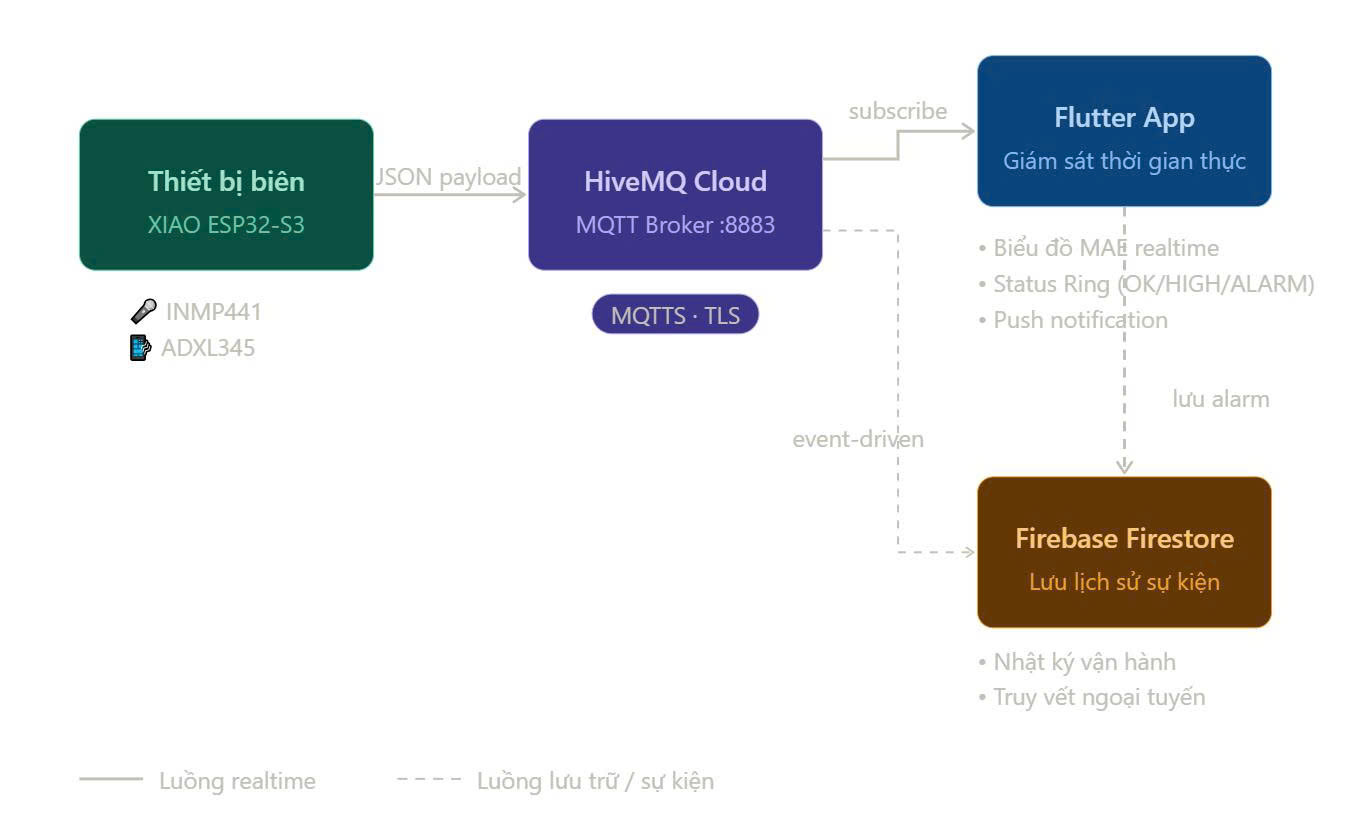
\includegraphics[width=0.85\textwidth]{chap4/image/app_architecture.png}
    \caption[Kiến trúc kết nối đám mây của ứng dụng di động]{Sơ đồ kiến trúc kết nối đám mây của ứng dụng di động. Dữ liệu từ thiết bị biên được phân phát theo hai nhánh độc lập: nhánh thời gian thực qua MQTT tới giao diện người dùng và nhánh lưu trữ lâu dài qua Firebase Firestore.}
    \label{fig:app_architecture}
\end{figure}

\textbf{HiveMQ Cloud} tiếp nhận luồng dữ liệu thời gian thực từ thiết bị biên với vai trò máy chủ trung gian MQTT. Dữ liệu được đóng gói theo định dạng JSON và truyền qua cổng 8883 (MQTTS), đảm bảo bảo mật và giữ độ trễ thấp.

\textbf{Firebase Firestore} lưu trữ lịch sử các sự kiện bất thường. Firestore là cơ sở dữ liệu NoSQL tổ chức dữ liệu theo các bộ sưu tập và tài liệu, phù hợp với dữ liệu vận hành có cấu trúc linh hoạt như thời điểm cảnh báo, pha vận hành, giá trị MAE và trạng thái xử lý \citeweb{ref_firestore_docs}. Người dùng có thể tra cứu nhật ký vận hành và mốc thời gian lỗi ngay cả khi thiết bị biên ngoại tuyến; điều này hỗ trợ bảo trì theo lịch.

% ============================================================
\subsection{Logic xử lý dữ liệu và thông báo đẩy}
% ============================================================

Ứng dụng sử dụng bộ lắng nghe MQTT để xử lý dữ liệu. Mỗi khi nhận gói tin từ chủ đề \texttt{tinyml/quang\_wm\_2026/status}, ứng dụng thực hiện ba bước: giải mã tải tin JSON để trích xuất các trường \texttt{is\_alarm}, \texttt{mae} và \texttt{mode}; kích hoạt thông báo đẩy ưu tiên cao nếu phát hiện cảnh báo, kèm đầy đủ giá trị MAE và pha vận hành; ghi nhận sự kiện vào Firestore. Song song đó, biểu đồ MAE trên giao diện được cập nhật liên tục.

Thông báo được tạo thông qua thư viện \texttt{flutter\_local\_notifications} với mức ưu tiên cao, bao gồm giá trị MAE và pha vận hành tại thời điểm xảy ra lỗi. Đo đạc độ trễ từ đầu đến cuối — từ khi vi điều khiển phát hiện bất thường đến khi thông báo xuất hiện — ghi nhận mức xấp xỉ \textbf{2,0 giây}. Thời gian này bao gồm độ trễ MQTT qua máy chủ trung gian và phản hồi của hệ điều hành, đáp ứng yêu cầu giám sát thời gian thực cho thiết bị gia dụng. Hình~\ref{fig:notification} minh họa thông báo đẩy trên Android.

\begin{figure}[H]
    \centering
    \begin{subfigure}[b]{0.42\textwidth}
        \centering
        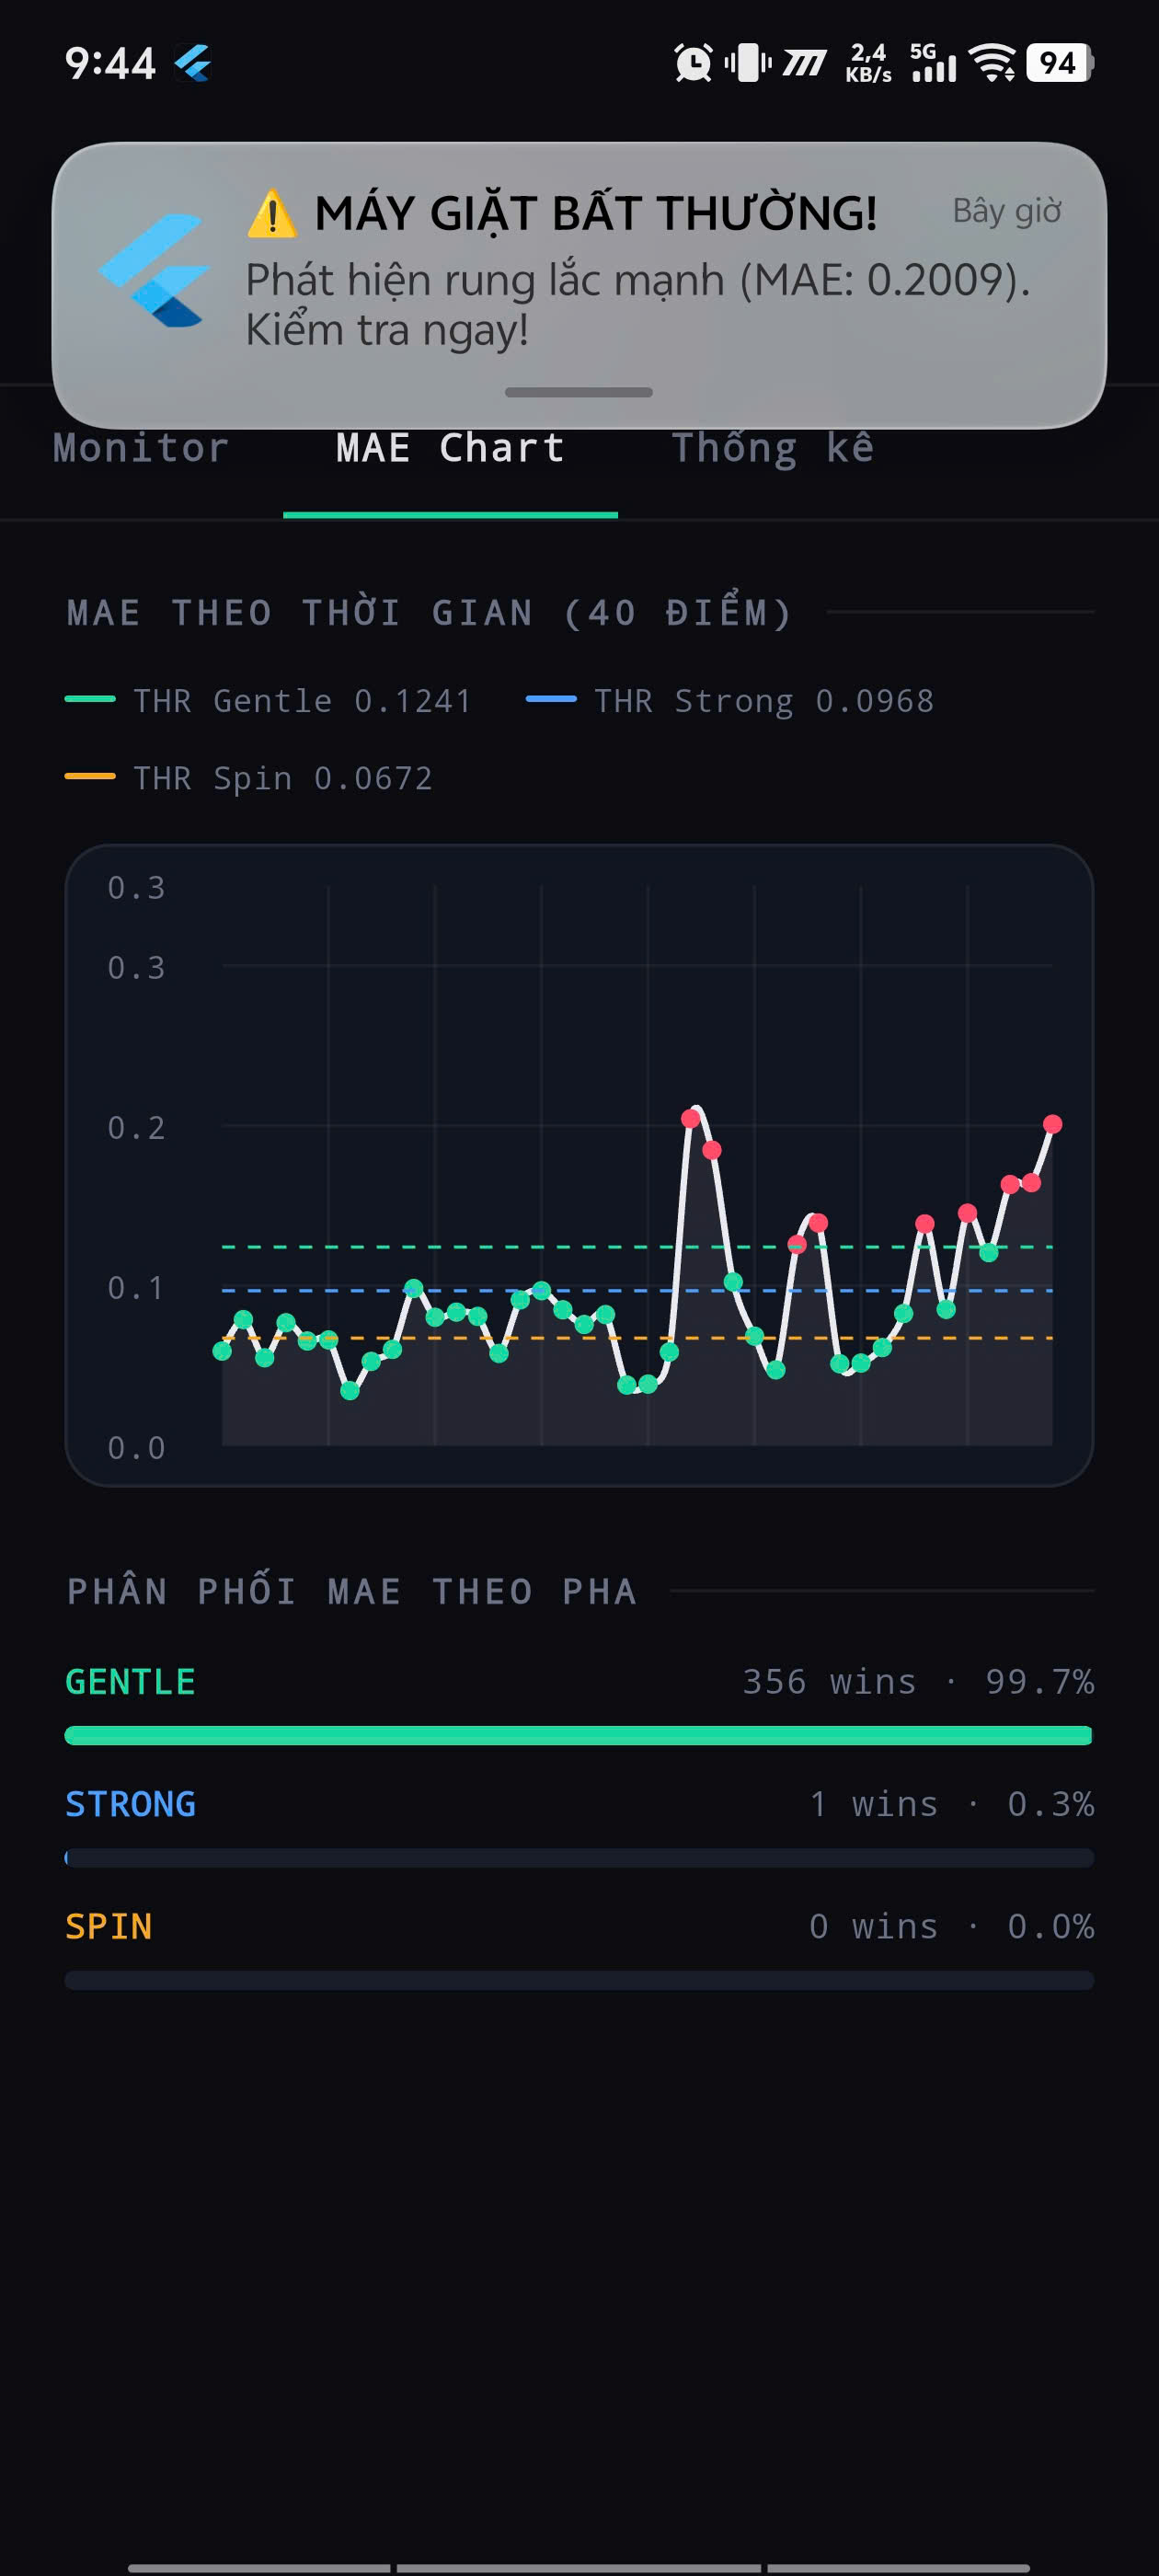
\includegraphics[width=\linewidth]{chap4/image/notification_banner.png}
        \caption{Thông báo dạng banner xuất hiện phía trên màn hình khi ứng dụng đang mở.}
        \label{fig:notif_banner}
    \end{subfigure}
    \hfill
    \begin{subfigure}[b]{0.42\textwidth}
        \centering
        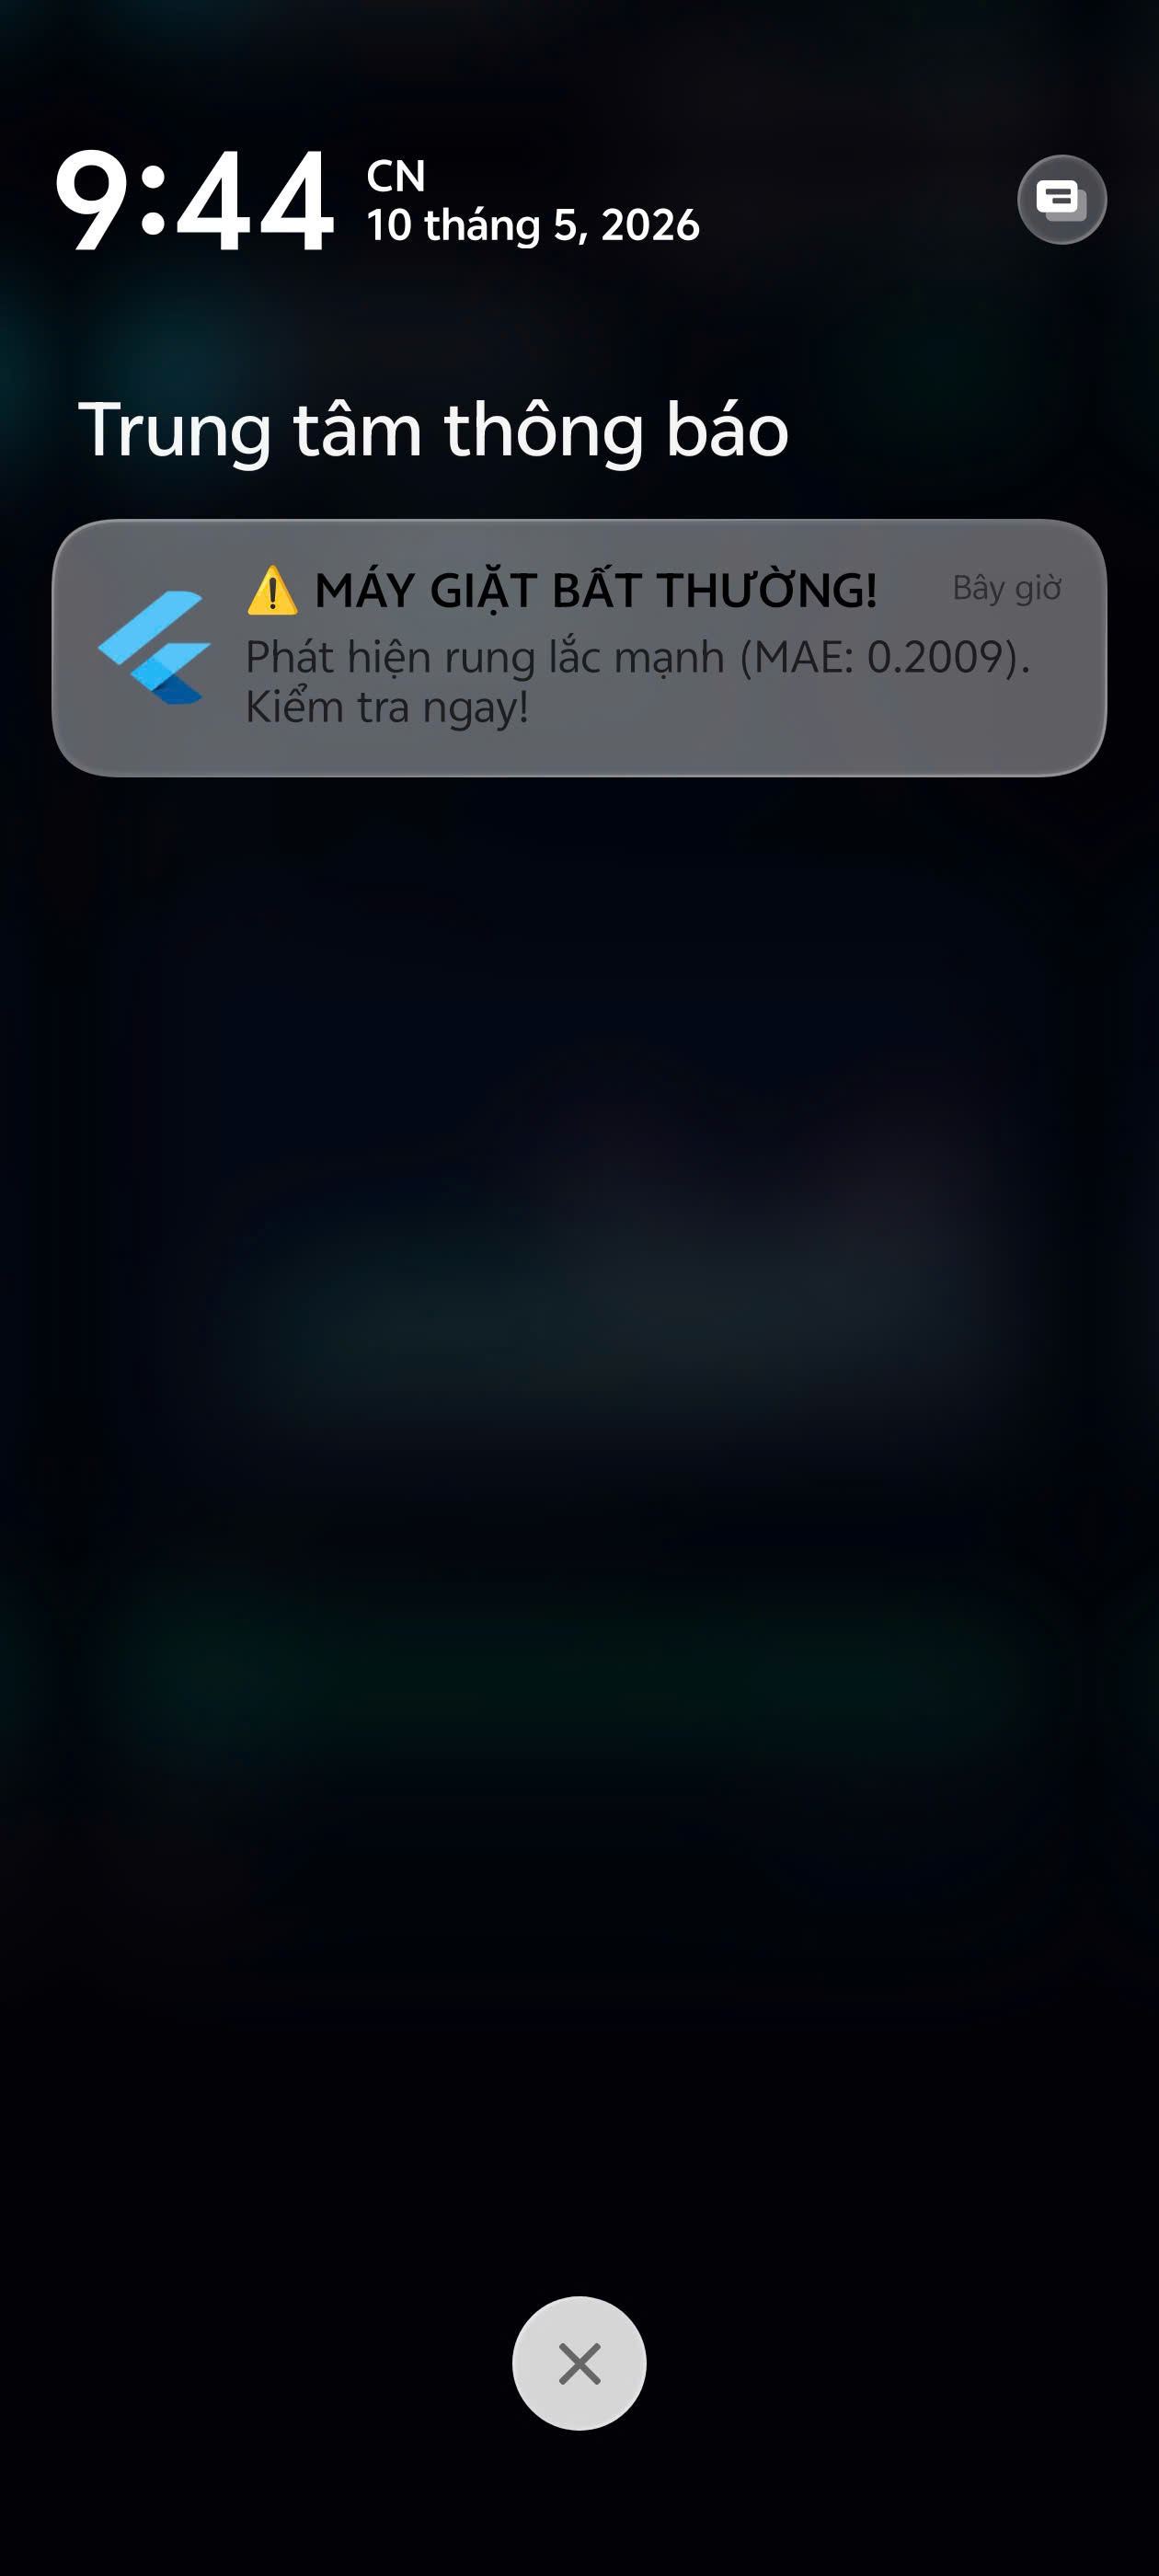
\includegraphics[width=\linewidth]{chap4/image/notification_lockscreen.png}
        \caption{Thông báo hiển thị tại Trung tâm thông báo khi thiết bị đang khóa màn hình.}
        \label{fig:notif_lockscreen}
    \end{subfigure}
    \caption[Minh họa thông báo đẩy trên Android]{Thông báo đẩy thực tế trên Android khi hệ thống kích hoạt ALARM --- "Phát hiện rung lắc mạnh (MAE: 0.2009). Kiểm tra ngay!". Thông báo được gửi trong vòng \textbf{2,0 giây} kể từ khi vi điều khiển phát hiện bất thường.}
    \label{fig:notification}
\end{figure}

\subsection{Giao diện người dùng và trực quan hóa dữ liệu}
% ============================================================

Giao diện sử dụng chế độ tối hiện đại, tổ chức thành ba phần chức năng như tại Hình~\ref{fig:app_ui}.

\begin{figure}[H]
    \centering
    \begin{subfigure}[b]{0.32\textwidth}
        \centering
        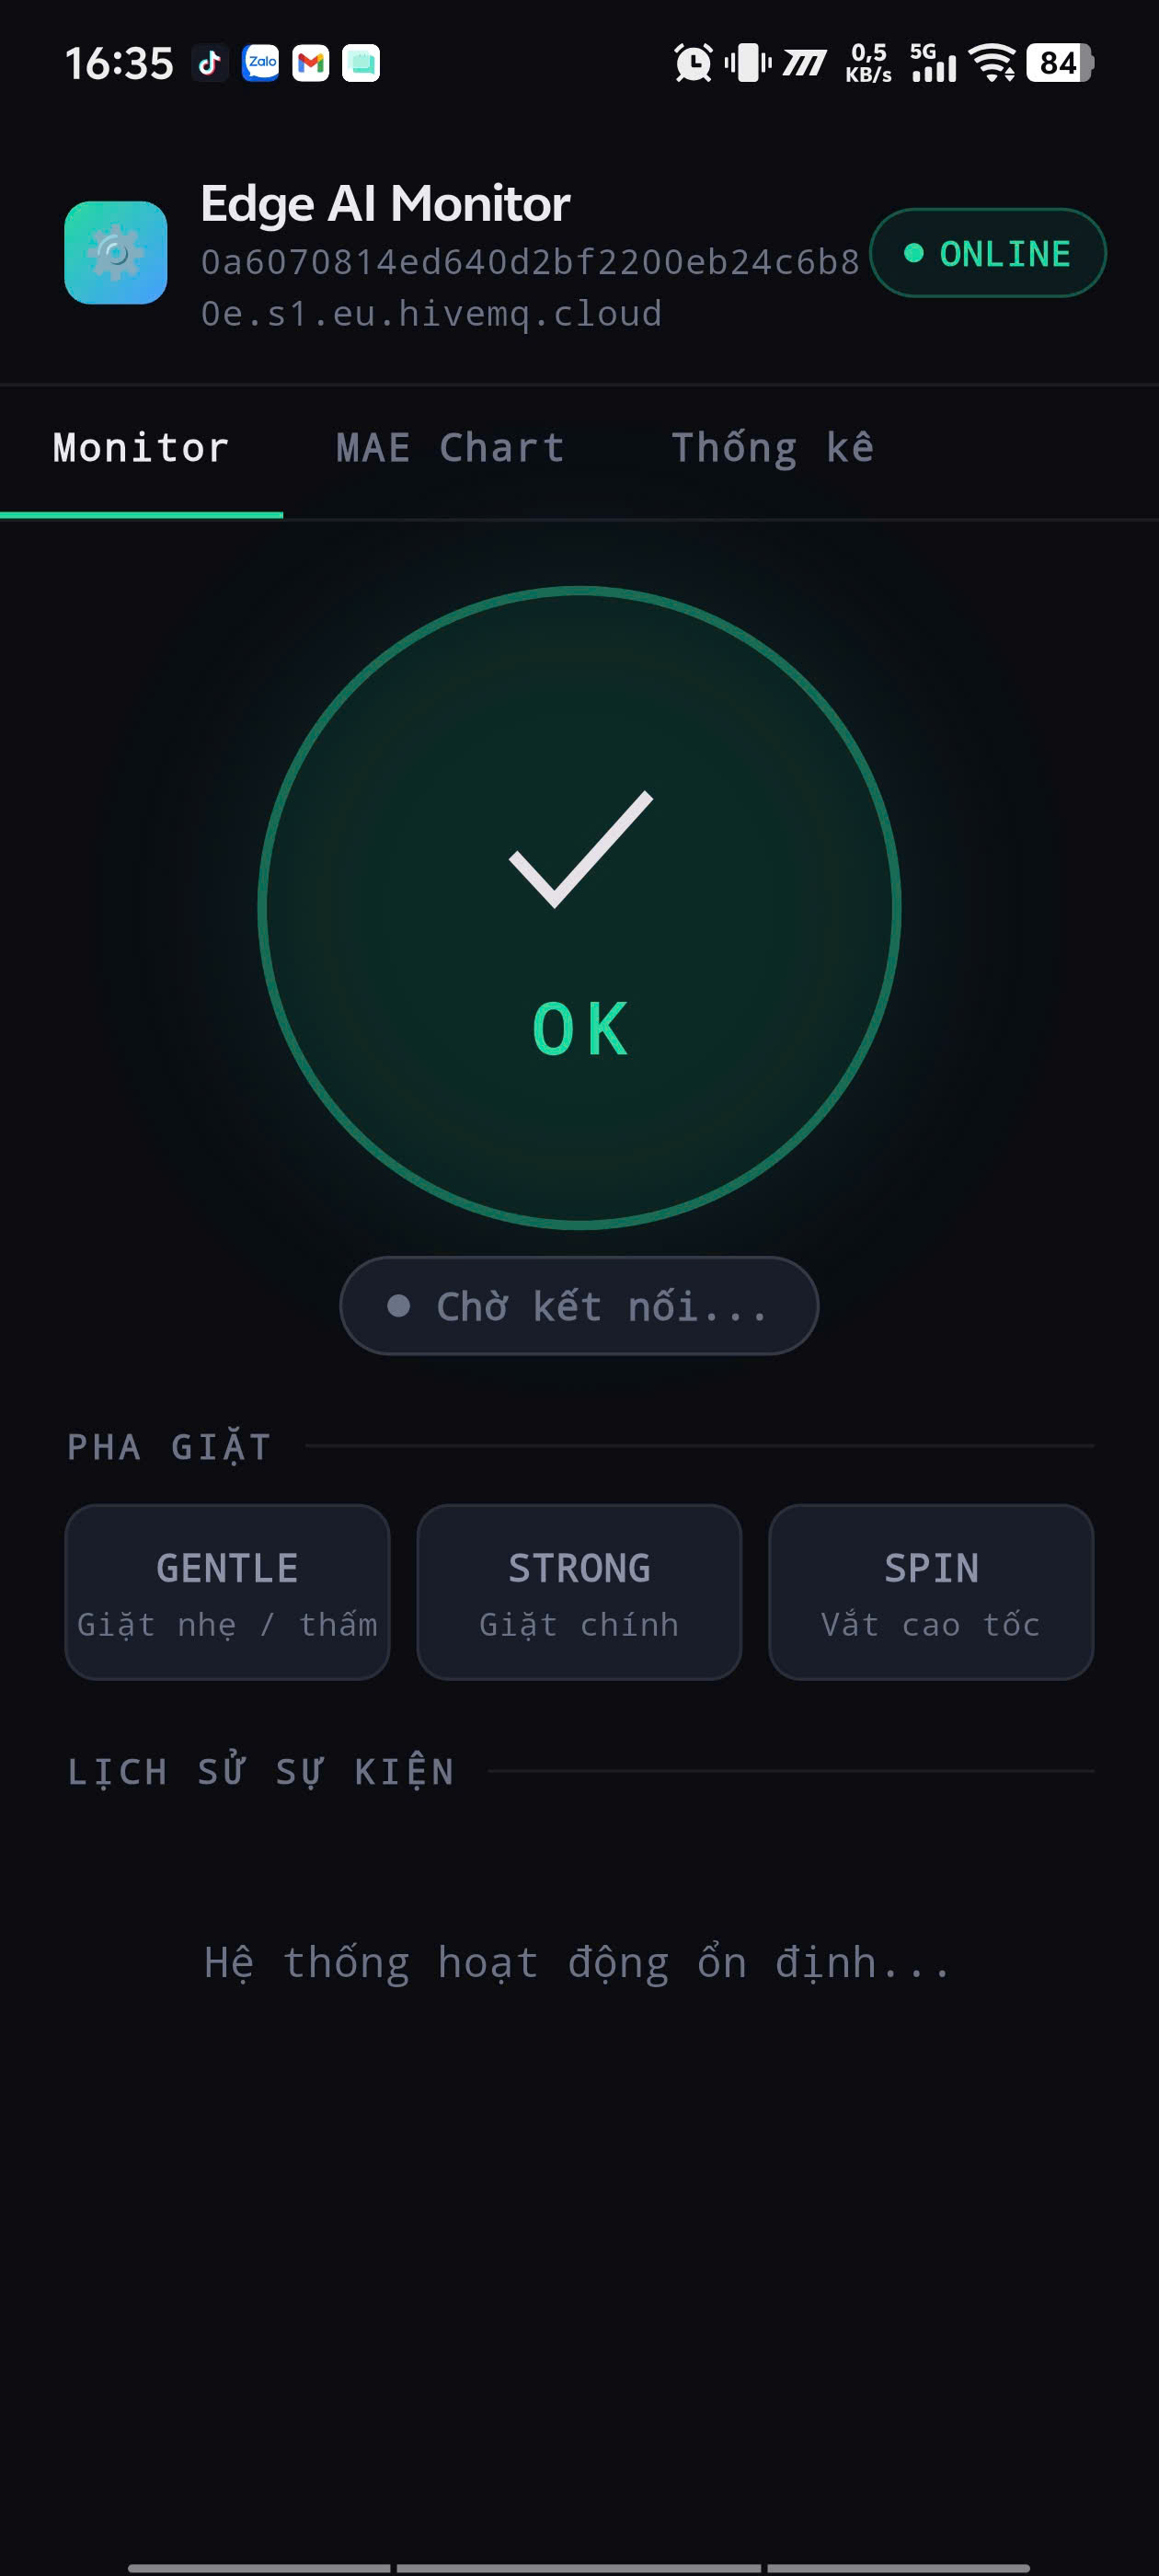
\includegraphics[width=\linewidth]{chap4/image/app_monitor.png}
        \caption{Màn hình Giám sát}
        \label{fig:ui_monitor}
    \end{subfigure}
    \hfill
    \begin{subfigure}[b]{0.32\textwidth}
        \centering
        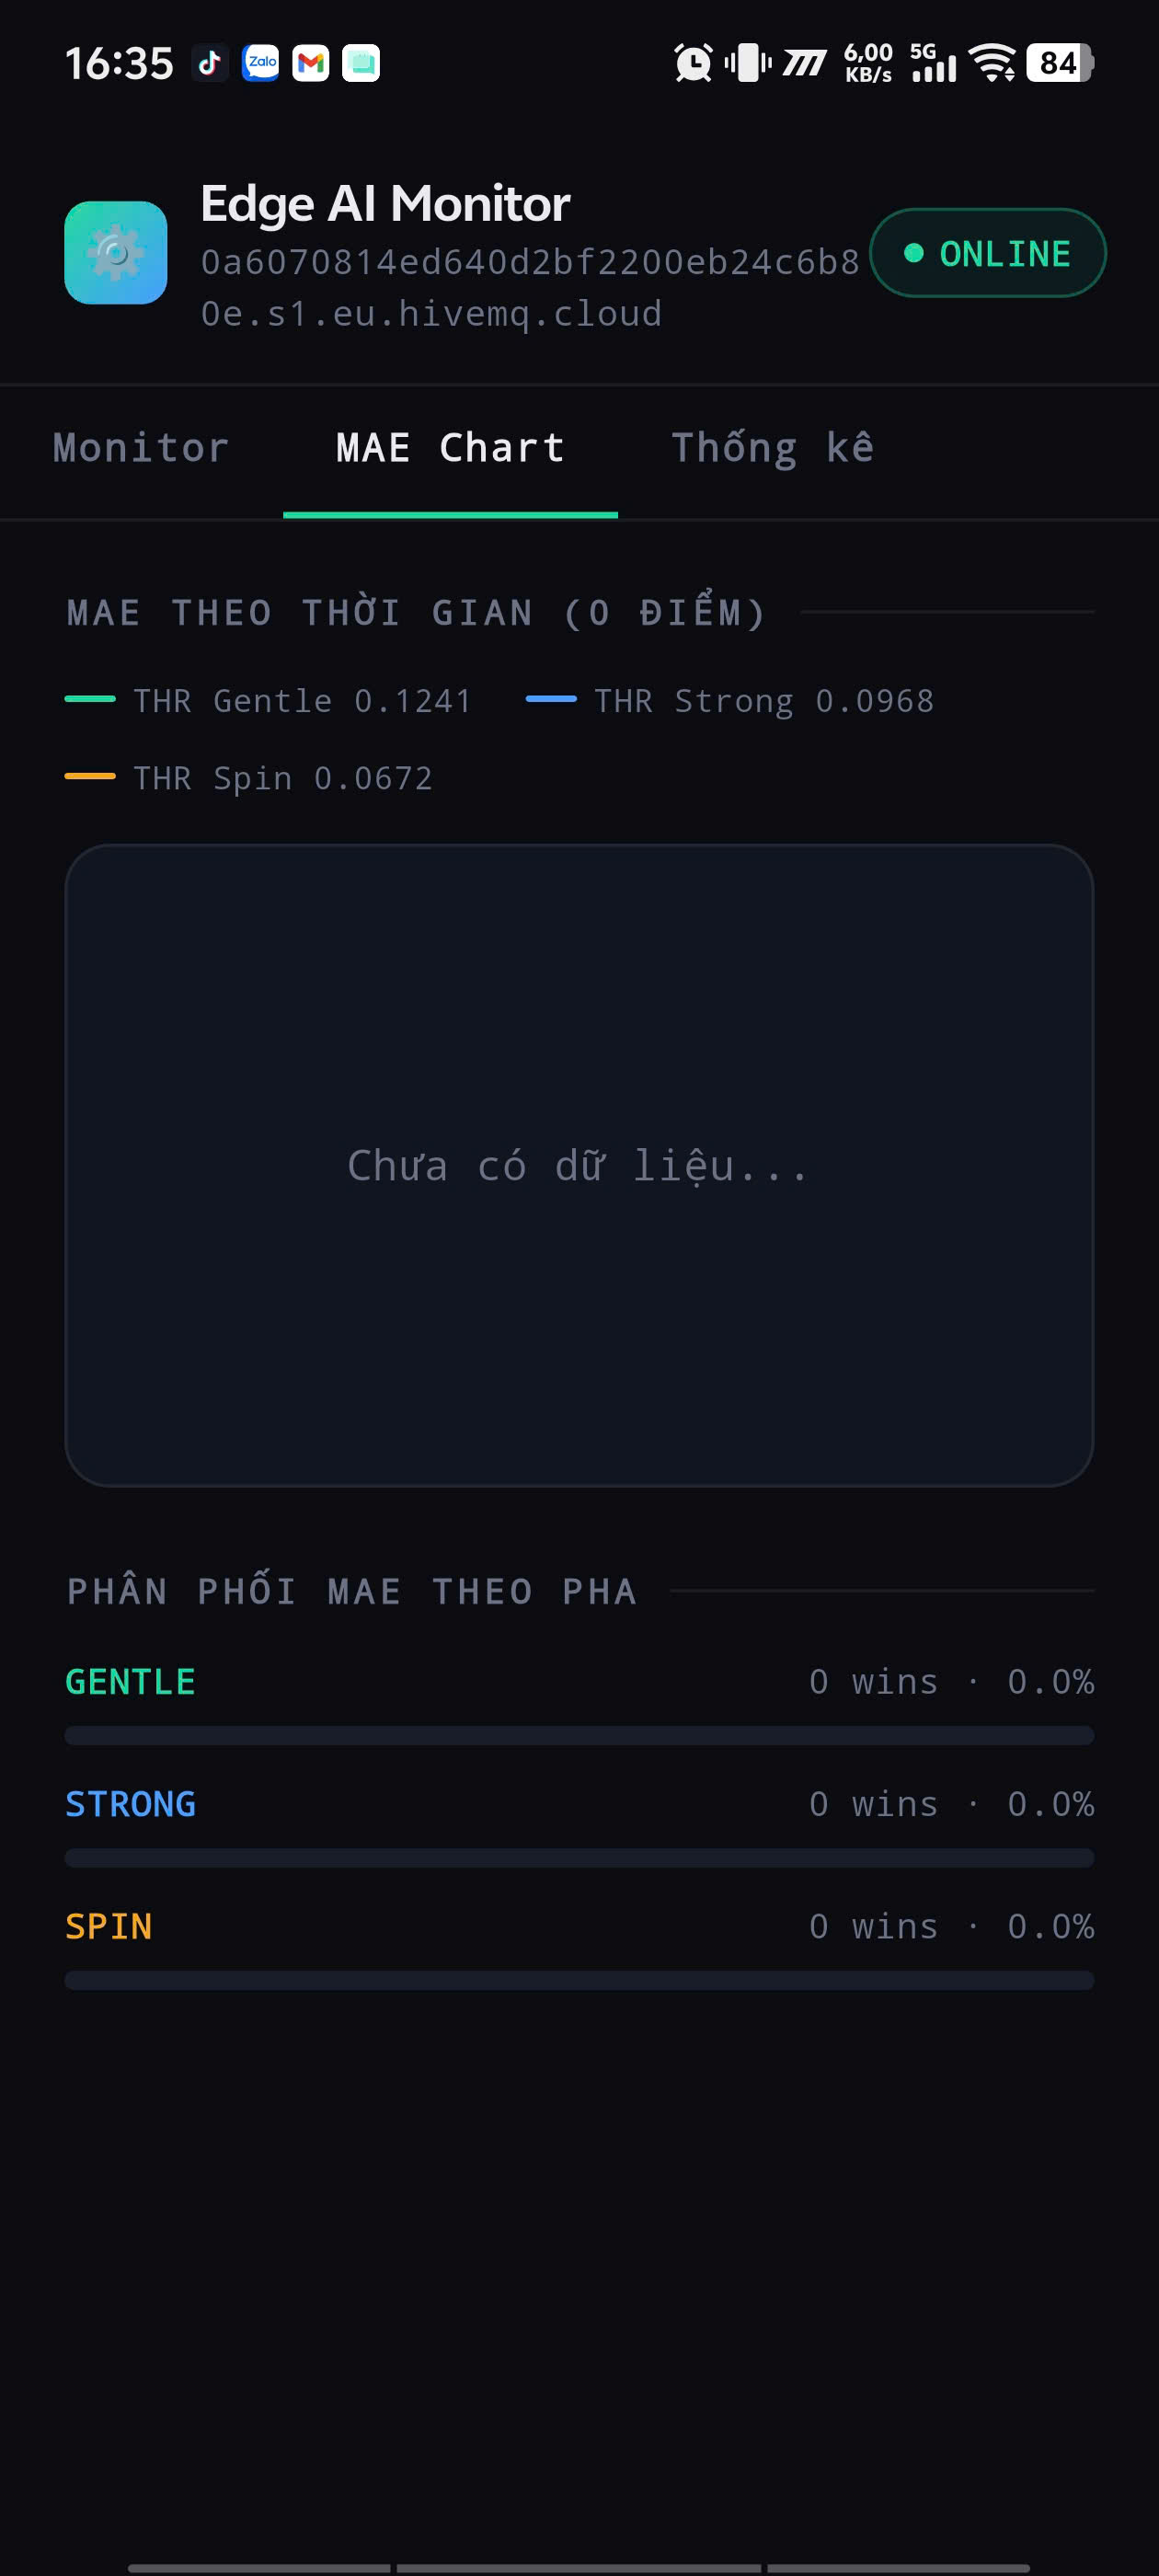
\includegraphics[width=\linewidth]{chap4/image/app_mae_chart.png}
        \caption{Biểu đồ MAE}
        \label{fig:ui_chart}
    \end{subfigure}
    \hfill
    \begin{subfigure}[b]{0.32\textwidth}
        \centering
        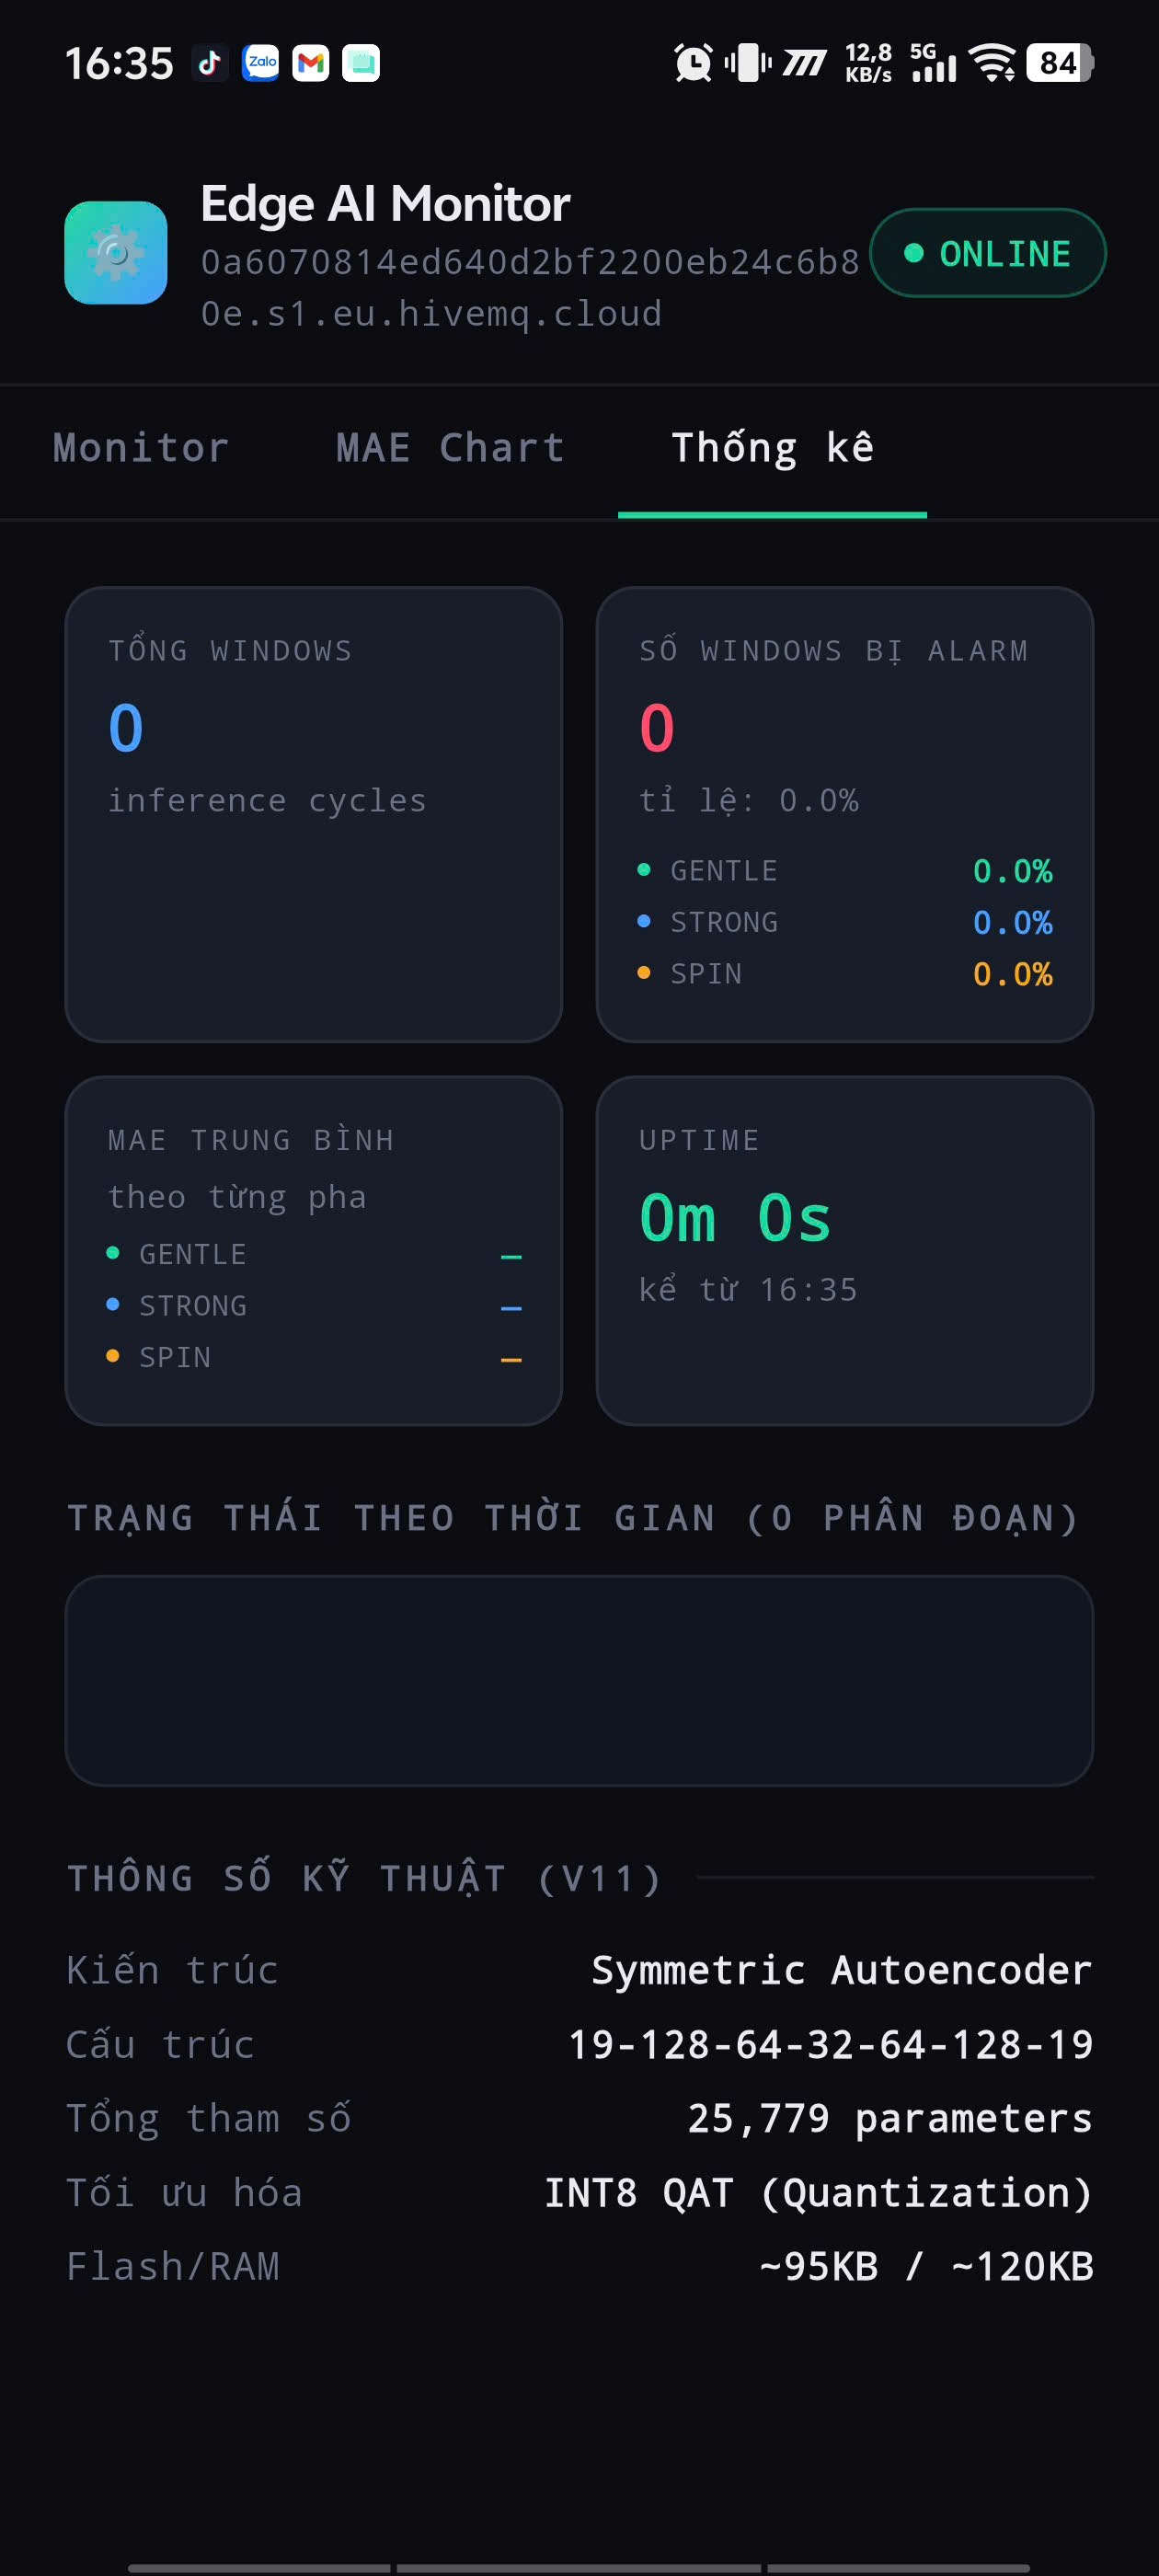
\includegraphics[width=\linewidth]{chap4/image/app_stats.png}
        \caption{Thống kê và Thông số}
        \label{fig:ui_stats}
    \end{subfigure}
    \caption[Giao diện ứng dụng di động Flutter]{Giao diện ứng dụng di động Flutter: (a) Vòng tròn trạng thái động; (b) Trực quan hóa sai số MAE cùng các đường ngưỡng $\tau$ tương ứng; (c) Bảng thống kê nhật ký vận hành và thông số mô hình thực tế.}
    \label{fig:app_ui}
\end{figure}

\textbf{Màn hình Giám sát (Monitor)} hiển thị vòng tròn trạng thái động thay đổi màu sắc: xanh lá ứng với trạng thái bình thường (OK), vàng khi sai số tiệm cận ngưỡng (HIGH), đỏ khi kích hoạt cảnh báo (ALARM). Cơ chế này giúp người dùng nhận biết tình trạng máy trong một cái nhìn mà không cần đọc số liệu kỹ thuật.

\textbf{Biểu đồ MAE thời gian thực} được dựng bằng thư viện \texttt{fl\_chart}, thể hiện sai số tái tạo theo thời gian. Đường ngưỡng $\tau$ tương ứng với pha vận hành hiện tại được vẽ chồng lên dạng đường đứt nét làm tham chiếu. Quan sát xu hướng MAE trước khi chạm ngưỡng có giá trị thực tiễn: người dùng có thể nhận diện sớm dấu hiệu bất thường đang tích lũy và kiểm tra thiết bị trước khi lỗi trở nên nghiêm trọng.

\textbf{Màn hình Thống kê và Nhật ký} tổng hợp số lượng cảnh báo theo từng pha vận hành (GENTLE, STRONG, SPIN), hỗ trợ người dùng đánh giá xu hướng hao mòn của thiết bị theo các chế độ giặt khác nhau trong dài hạn.

Lớp ứng dụng di động này hoàn thiện vòng phản hồi của hệ thống AIoT và kết nối các thuật toán TinyML phức tạp với người dùng cuối, giúp các chỉ số kỹ thuật trở thành thông tin cảnh báo có ý nghĩa thực tiễn và dễ tiếp cận.
